\documentclass[11pt,a4paper]{article}
\usepackage[utf8]{inputenc}
\usepackage[T1]{fontenc}
\usepackage[brazil]{babel}
\usepackage{lmodern}
\usepackage[margin=2.5cm]{geometry}
\usepackage{graphicx}
\usepackage{listings}
\usepackage{xcolor}
\usepackage{booktabs}
\usepackage{longtable}
\usepackage{array}
\usepackage{float}
\usepackage[colorlinks=true,linkcolor=blue!50!black,urlcolor=blue!50!black]{hyperref}

\lstset{
  basicstyle=\ttfamily\small,
  breaklines=true,
  frame=single,
  backgroundcolor=\color{gray!8},
  columns=fullflexible,
  keepspaces=true,
  upquote=true,
  literate={á}{{\'a}}1 {é}{{\'e}}1 {í}{{\'i}}1 {ó}{{\'o}}1 {ú}{{\'u}}1
           {ã}{{\~a}}1 {õ}{{\~o}}1 {ç}{{\c c}}1 {â}{{\^a}}1 {ê}{{\^e}}1
}

\newcommand{\code}[1]{\texttt{\detokenize{#1}}}

\title{\textbf{k230\_updater}\\[2pt]\large Biblioteca MicroPython para CanMV K230:\\
atualiza\c{c}\~ao remota, salva-guarda com watchdog e controle t\'ermico}
\author{Documenta\c{c}\~ao t\'ecnica}
\date{\today}

\begin{document}
\maketitle
\tableofcontents
\newpage

%------------------------------------------------------------------
\section{Introdu\c{c}\~ao}
A biblioteca \code{k230_updater} foi escrita para placas \textbf{CanMV K230} (MicroPython) que operam em campo e precisam:
\begin{enumerate}
  \item receber novas vers\~oes do programa (\code{main.py}) e de modelos \code{.kmodel} remotamente, a partir de um reposit\'orio GitHub \textbf{privado} ou de um servidor HTTP que entrega um arquivo \code{.zip};
  \item sobreviver a uma vers\~ao defeituosa gra\c{c}as a um \textbf{watchdog de hardware}, com rollback autom\'atico e possibilidade de receber uma vers\~ao corrigida;
  \item limitar a temperatura do chip reduzindo a taxa de quadros (FPS) da captura.
\end{enumerate}

\paragraph{Status.} O c\'odigo foi escrito e revisado sem execu\c{c}\~ao em hardware. Apenas o extrator de zip foi testado em um PC. Antes do uso em produ\c{c}\~ao, valide no seu firmware: a API de \code{machine.WDT}, o suporte HTTPS do m\'odulo \code{requests}, \code{machine.chipid()} e a leitura de temperatura.

%------------------------------------------------------------------
\section{Vis\~ao geral da arquitetura}
A Figura~\ref{fig:blocos} mostra os blocos da solu\c{c}\~ao e o fluxo entre eles.

\begin{figure}[H]
  \centering
  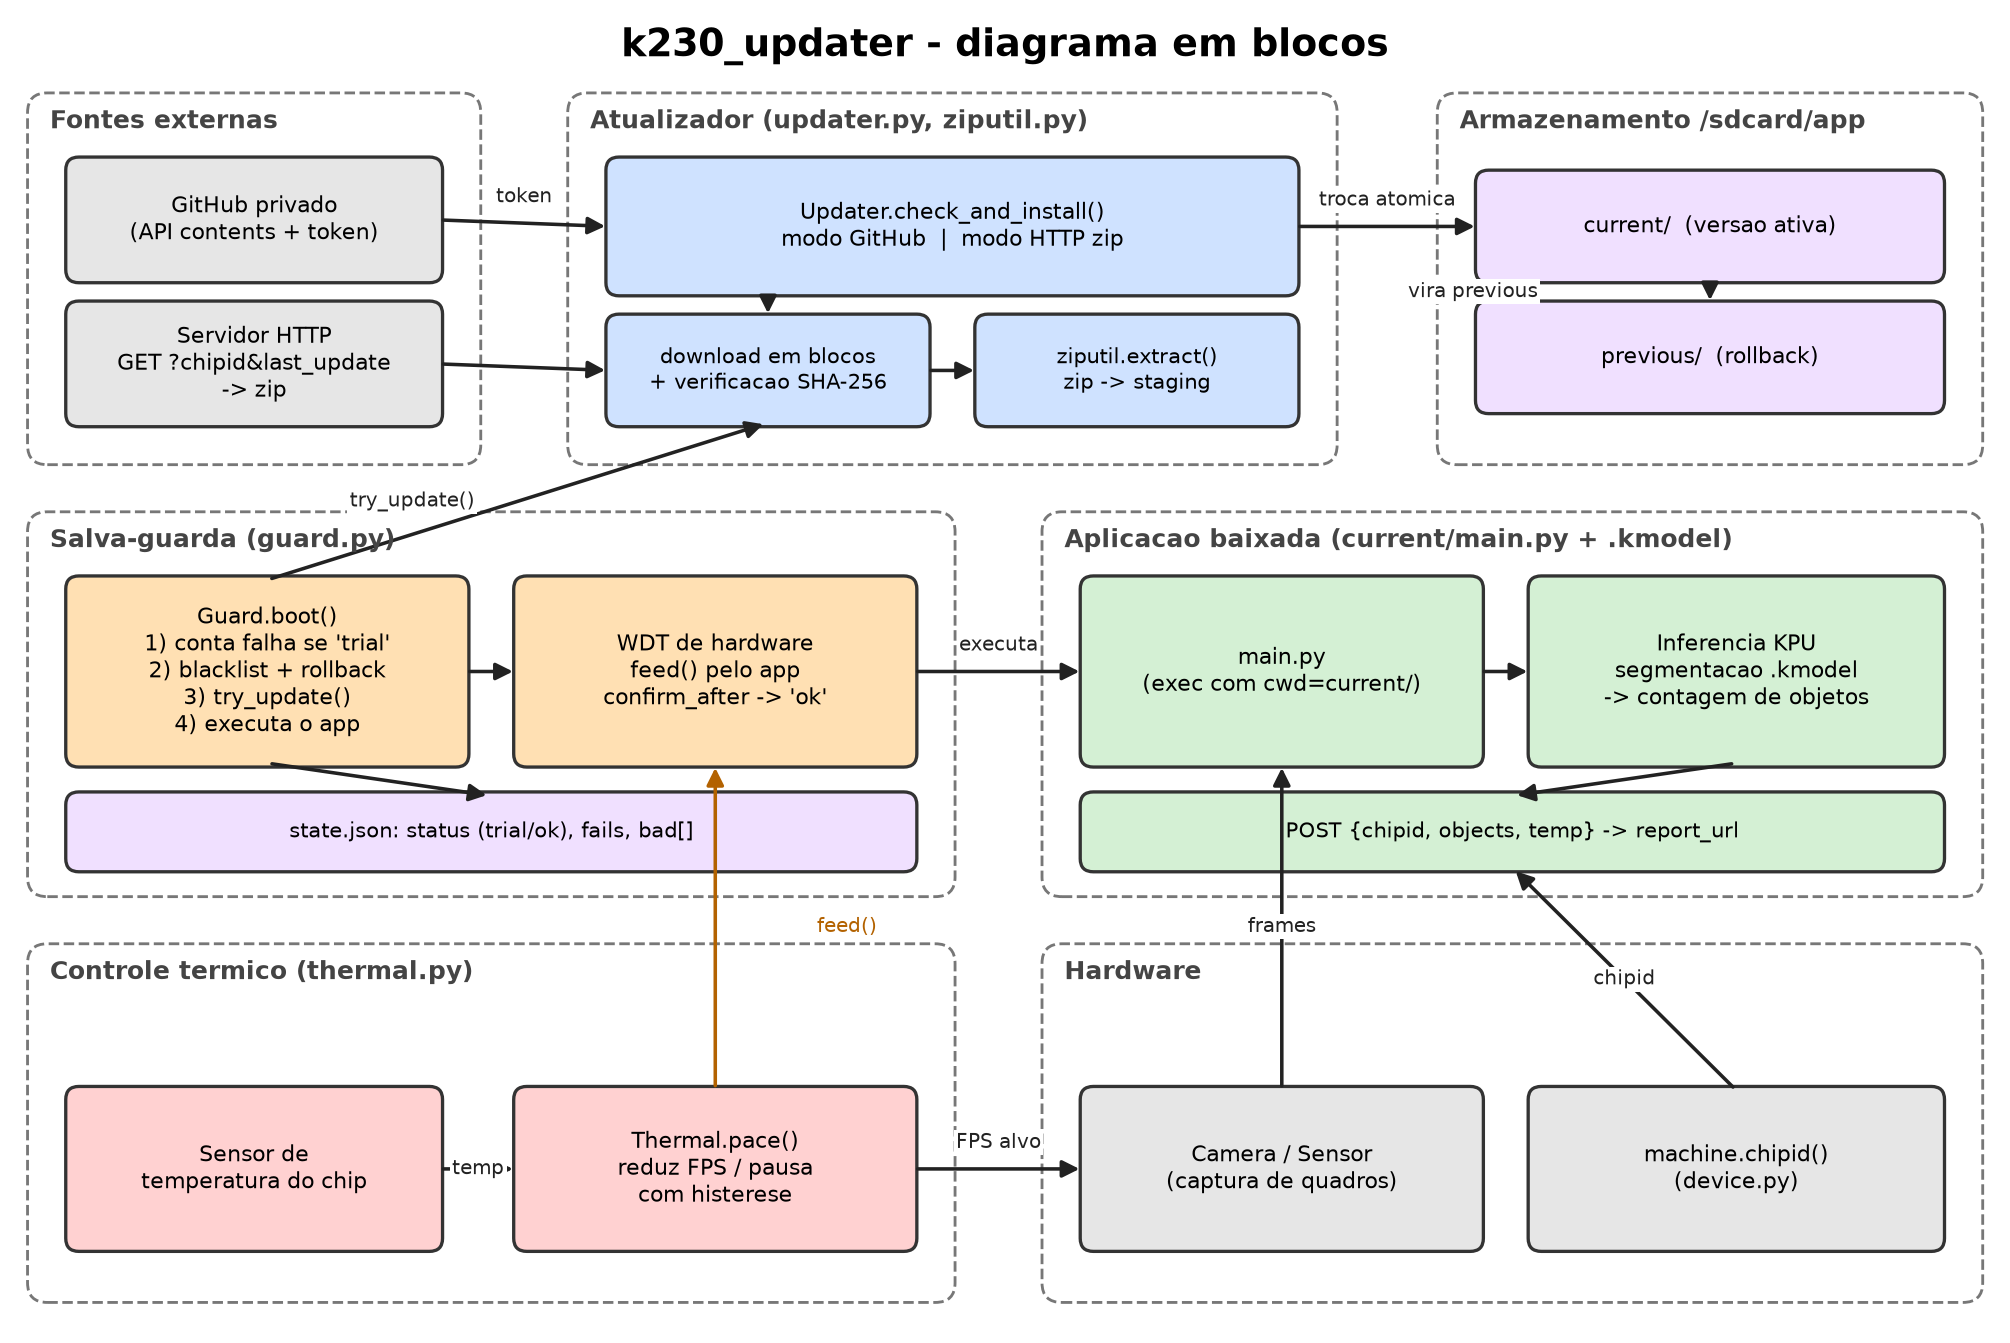
\includegraphics[width=\textwidth]{figs/diagrama_blocos.png}
  \caption{Diagrama em blocos do \code{k230_updater}.}
  \label{fig:blocos}
\end{figure}

\subsection{M\'odulos}
\begin{longtable}{@{}p{3.6cm}p{11.4cm}@{}}
\toprule
\textbf{Arquivo} & \textbf{Responsabilidade}\\
\midrule
\endhead
\code{main.py} (raiz) & Launcher permanente gravado no cart\~ao SD. L\^e o \code{config.json}, cria o \code{Guard} e chama \code{boot()}. N\~ao \'e atualizado remotamente.\\
\code{k230_updater/guard.py} & Salva-guarda: watchdog, estado \emph{trial/ok}, contagem de falhas, lista de vers\~oes proibidas, rollback e execu\c{c}\~ao do aplicativo.\\
\code{k230_updater/updater.py} & Busca e instala vers\~oes (modo GitHub ou modo HTTP/zip), verifica SHA-256, troca at\^omica de diret\'orios.\\
\code{k230_updater/ziputil.py} & Extrator de zip para MicroPython (sem depender de \code{zipfile}).\\
\code{k230_updater/thermal.py} & Governador t\'ermico: ajusta o FPS conforme a temperatura.\\
\code{k230_updater/device.py} & Fun\c{c}\~ao \code{chip_id()} (identificador \'unico do K230 em hexadecimal).\\
\code{k230_updater/util.py} & Utilit\'arios de arquivos: \code{makedirs}, \code{rmtree}, JSON com grava\c{c}\~ao segura.\\
\code{examples/} & Aplicativo de exemplo, aplicativo de segmenta\c{c}\~ao e servidor de refer\^encia para PC.\\
\bottomrule
\end{longtable}

%------------------------------------------------------------------
\section{Instala\c{c}\~ao e configura\c{c}\~ao}
\subsection{Layout do cart\~ao SD}
\begin{lstlisting}
/sdcard/main.py            launcher permanente
/sdcard/config.json        configuracao (contem o token: mantenha secreto)
/sdcard/k230_updater/      a biblioteca
/sdcard/app/               criado automaticamente
    current/               versao em execucao
    previous/              versao anterior (alvo do rollback)
    staging/               download temporario
    state.json             estado do salva-guarda
\end{lstlisting}

\subsection{Arquivo \texttt{config.json}}
\begin{longtable}{@{}p{3.2cm}p{2.3cm}p{9.5cm}@{}}
\toprule
\textbf{Campo} & \textbf{Padr\~ao} & \textbf{Descri\c{c}\~ao}\\
\midrule
\endhead
\code{repo} & --- & Reposit\'orio privado, formato \code{dono/repositorio} (modo GitHub).\\
\code{token} & --- & Token \emph{fine-grained} com permiss\~ao \textbf{Contents: Read-only} restrita a esse reposit\'orio. No modo HTTP, se informado, \'e enviado como \code{Authorization: Bearer}.\\
\code{branch} & \code{main} & Branch consultada (modo GitHub).\\
\code{update_url} & vazio & Se definido, ativa o modo HTTP/zip (se\c{c}\~ao~\ref{sec:http}).\\
\code{report_url} & --- & URL do \code{POST} usado pelo exemplo de segmenta\c{c}\~ao.\\
\code{wdt_timeout} & 10 & Timeout do watchdog em segundos.\\
\code{max_fails} & 3 & Falhas consecutivas antes de proibir a vers\~ao e voltar \`a anterior.\\
\code{confirm_after} & 60 & Segundos alimentando o watchdog at\'e a vers\~ao ser considerada boa.\\
\bottomrule
\end{longtable}
Edite a fun\c{c}\~ao \code{connect()} do \code{main.py} para o seu meio de rede (Ethernet ou Wi-Fi). Nunca versione o \code{config.json}.

%------------------------------------------------------------------
\section{Fontes de atualiza\c{c}\~ao}
\subsection{Modo GitHub (reposit\'orio privado)}
O reposit\'orio deve conter um \code{manifest.json} e os arquivos listados:
\begin{lstlisting}
{
  "version": "1.0.1",
  "entry": "main.py",
  "files": [
    {"path": "main.py", "sha256": "<hex>"},
    {"path": "models/detector.kmodel", "sha256": "<hex>"}
  ]
}
\end{lstlisting}
\begin{itemize}
  \item \code{version}: texto comparado por igualdade; \textbf{altere a cada release}.
  \item \code{entry}: arquivo executado (padr\~ao \code{main.py}).
  \item \code{sha256}: recomendado; se divergir, a instala\c{c}\~ao \'e abortada e \code{current} permanece intacto.
\end{itemize}
Cada arquivo \'e obtido por \code{GET https://api.github.com/repos/<repo>/contents/<path>?ref=<branch>} com o cabe\c{c}alho \code{Accept: application/vnd.github.raw+json}, e gravado em blocos de 4~KiB, alimentando o watchdog durante o download.

\subsection{Modo HTTP com pacote zip}\label{sec:http}
Com \code{update_url} definido, a cada verifica\c{c}\~ao a placa executa:
\begin{lstlisting}
GET <update_url>?chipid=<id hex do K230>&last_update=<data da ultima atualizacao>
\end{lstlisting}
\begin{itemize}
  \item \code{last_update} \'e o campo \code{updated_at} do manifesto instalado (vazio se n\~ao h\'a nada instalado), codificado como URL.
  \item Resposta \textbf{204} ou \textbf{304}: nada a fazer. Resposta \textbf{200}: o corpo \'e um zip com \code{main.py}, \code{models/*.kmodel} etc.
  \item A vers\~ao vem do \code{manifest.json} dentro do zip (opcional) ou do cabe\c{c}alho \code{X-Version}. A data vem do manifesto ou de \code{X-Updated-At}; na falta de ambos, usa-se a hora local da placa. Sem nenhuma vers\~ao, a atualiza\c{c}\~ao falha.
  \item Vers\~oes na lista de proibidas s\~ao descartadas depois do download.
  \item Entradas com caminho absoluto, com \code{..} ou com barra invertida s\~ao rejeitadas.
\end{itemize}
\paragraph{Zip e mem\'oria.} Entradas \emph{stored} (m\'etodo 0) s\~ao copiadas em blocos; para modelos grandes crie o zip \textbf{sem compress\~ao} (\code{zip -0}). Entradas \emph{deflate} (m\'etodo 8) s\~ao lidas inteiras na RAM e exigem \code{deflate}, \code{zlib} ou \code{uzlib} no firmware.

\subsection{Troca at\^omica e integridade}
Em ambos os modos o pacote \'e primeiro montado em \code{staging/}. Somente ap\'os todos os arquivos serem baixados e verificados \'e feita a troca:
\begin{enumerate}
  \item \code{previous/} \'e removido;
  \item \code{current/} \'e renomeado para \code{previous/};
  \item \code{staging/} \'e renomeado para \code{current/}.
\end{enumerate}
Qualquer falha antes da troca remove \code{staging/} e n\~ao afeta a vers\~ao ativa. O \code{state.json} \'e gravado em arquivo tempor\'ario e renomeado.

%------------------------------------------------------------------
\section{Salva-guarda com watchdog}
\subsection{Conceito}
O watchdog de hardware (\code{machine.WDT}) \'e alimentado apenas pelo aplicativo, por meio de \code{guard.feed()} (ou \code{Thermal.pace()}). Se o aplicativo travar, o watchdog reinicia a placa. Uma vers\~ao nova \'e considerada \emph{em teste} (\textit{trial}) at\'e alimentar o watchdog durante \code{confirm_after} segundos; ent\~ao passa a \textit{ok}.

\subsection{Fluxo de boot}
\begin{enumerate}
  \item Inicia o watchdog.
  \item Se o estado salvo for \textit{trial}, a execu\c{c}\~ao anterior n\~ao foi confirmada: conta uma falha. Ao atingir \code{max_fails}, a vers\~ao atual entra na lista \code{bad} e \code{previous/} \'e restaurado.
  \item Chama \code{try_update()}: instala qualquer vers\~ao nova que n\~ao esteja proibida. Isto ocorre \textbf{antes} de executar o aplicativo, de modo que uma corre\c{c}\~ao publicada recupera uma placa em ciclo de reinicializa\c{c}\~oes.
  \item Se n\~ao h\'a vers\~ao execut\'avel (nada instalado ou s\'o vers\~oes proibidas), aguarda \code{retry_interval} segundos alimentando o watchdog e tenta atualizar de novo.
  \item Marca \textit{trial}, grava o estado e executa o \code{entry} em \code{current/} (com \code{cwd} e \code{sys.path} apontando para \code{current/}).
\end{enumerate}
Ap\'os a execu\c{c}\~ao: exce\c{c}\~ao n\~ao tratada incrementa as falhas e reinicia; retorno normal tamb\'em reinicia (o aplicativo deve rodar indefinidamente); \code{KeyboardInterrupt} para o watchdog e restaura o estado \textit{ok}, para facilitar a depura\c{c}\~ao.

\subsection{Atualiza\c{c}\~ao corretiva}
Uma vers\~ao proibida nunca \'e reinstalada, mas \textbf{qualquer vers\~ao com identificador diferente} \'e. Para corrigir uma vers\~ao defeituosa (por exemplo, a \code{1.0.1}), publique a \code{1.0.2}. O aplicativo tamb\'em pode chamar \code{guard.update_and_reset()} periodicamente.

\subsection{Limita\c{c}\~oes}
\begin{itemize}
  \item Se o launcher ou a biblioteca tiverem defeito, n\~ao h\'a recupera\c{c}\~ao remota: mantenha-os m\'inimos e testados.
  \item Sem rede, com a vers\~ao atual proibida e sem \code{previous/}, a placa fica aguardando sem executar o aplicativo.
  \item Carregar um modelo grande pode exceder \code{wdt_timeout}: aumente-o ou alimente o watchdog antes e depois do carregamento.
\end{itemize}

%------------------------------------------------------------------
\section{Controle t\'ermico}
\code{Thermal} limita a temperatura ajustando o FPS. Use-o no la\c{c}o de captura:
\begin{lstlisting}[language=Python]
gov = Thermal(max_temp=75, target_fps=30, min_fps=2, feed=guard.feed)
while True:
    img = sensor.snapshot()
    # ... inferencia ...
    gov.pace()    # mantem o FPS, adapta a temperatura e alimenta o WDT
\end{lstlisting}
A temperatura \'e lida a cada \code{interval_ms} (padr\~ao 2000~ms):
\begin{center}
\begin{tabular}{@{}ll@{}}
\toprule
\textbf{Condi\c{c}\~ao} & \textbf{A\c{c}\~ao}\\
\midrule
$T \ge$ \code{max_temp + critical_margin} & N\'ivel 2: pausa a captura (alimentando o WDT) at\'e $T \le$ \code{max_temp - hysteresis}\\
$T \ge$ \code{max_temp} & FPS $\times 0{,}7$ (m\'inimo \code{min_fps}); n\'ivel 1\\
$T \le$ \code{max_temp - hysteresis} & FPS $\times 1{,}15$ at\'e \code{target_fps}; n\'ivel 0\\
caso contr\'ario & mant\'em o FPS\\
\bottomrule
\end{tabular}
\end{center}
\paragraph{Par\^ametros.} \code{max_temp}, \code{target_fps}, \code{min_fps=1}, \code{hysteresis=3}, \code{critical_margin=5}, \code{interval_ms=2000}, \code{read=None}, \code{feed=None}, \code{on_throttle=None}.
\begin{itemize}
  \item \code{read}: fun\c{c}\~ao que devolve a temperatura em graus Celsius. Se omitida, a biblioteca tenta \code{machine.temperature} e \code{machine.TSENSOR}; se nenhuma existir, levanta \code{RuntimeError}.
  \item \code{on_throttle(level)}: chamado quando o n\'ivel muda (0 normal, 1 reduzido, 2 pausado). Use-o para reduzir a frequ\^encia da CPU/KPU ou desligar perif\'ericos; a biblioteca n\~ao altera frequ\^encias por conta pr\'opria.
\end{itemize}

%------------------------------------------------------------------
\section{Refer\^encia da API}
\subsection{\texttt{Guard}}
\begin{lstlisting}[language=Python]
Guard(repo, token, root="/sdcard/app", branch="main", wdt_timeout=10,
      wdt_id=1, max_fails=3, confirm_after=60, retry_interval=60,
      connect=None, update_url=None)
\end{lstlisting}
\begin{longtable}{@{}p{4.2cm}p{10.8cm}@{}}
\toprule
\textbf{M\'etodo} & \textbf{Descri\c{c}\~ao}\\
\midrule
\endhead
\code{boot()} & Fluxo completo da se\c{c}\~ao~5.2; n\~ao retorna normalmente.\\
\code{feed()} & Alimenta o WDT e confirma a vers\~ao ap\'os \code{confirm_after} segundos.\\
\code{confirm()} & Confirma a vers\~ao atual manualmente.\\
\code{try_update()} & Verifica e instala atualiza\c{c}\~ao; nunca levanta exce\c{c}\~ao; devolve a vers\~ao instalada ou \code{None}.\\
\code{update_and_reset()} & Executa \code{try_update()} e reinicia se algo foi instalado.\\
\code{reset()} & Chama \code{machine.reset()}.\\
\code{start_wdt()}, \code{stop_wdt()} & Controle do watchdog.\\
\bottomrule
\end{longtable}
Dentro do aplicativo: \code{import k230_updater; guard = k230_updater.guard}.

\subsection{\texttt{Updater}}
\code{Updater(repo, token, root, branch, feed, url=None)} com os m\'etodos \code{remote_manifest()}, \code{local_manifest()}, \code{install(manifest)}, \code{check_and_install(skip_versions=())} e \code{rollback()}. Levanta \code{UpdateError} em HTTP diferente de 200, manifesto inv\'alido, hash divergente ou pacote sem vers\~ao.

\subsection{\texttt{Thermal}}
M\'etodos \code{pace()} e \code{update()}; atributos \code{fps}, \code{temp} e \code{level}.

\subsection{Utilit\'arios}
\code{device.chip_id()} devolve o identificador hexadecimal de \code{machine.chipid()}; \code{ziputil.extract(zip_path, dest, feed=None)} extrai um zip e devolve a lista de nomes.

%------------------------------------------------------------------
\section{Exemplo completo: segmenta\c{c}\~ao e relat\'orio}
O arquivo \code{examples/segmentation_app/main.py} \'e um aplicativo para ser publicado dentro do pacote de atualiza\c{c}\~ao, junto com \code{models/yolov8n_seg.kmodel}. Ele:
\begin{enumerate}
  \item inicializa a c\^amera e o runtime \code{nncase_runtime}, alimentando o watchdog antes e depois de carregar o \code{.kmodel};
  \item executa infer\^encia de segmenta\c{c}\~ao (estilo YOLOv8-seg), aplica NMS e calcula a \'area das m\'ascaras;
  \item usa \code{Thermal.pace()} para controlar o FPS conforme a temperatura;
  \item a cada \code{REPORT_EVERY_S} segundos envia um \code{POST} JSON para \code{report_url}:
\end{enumerate}
\begin{lstlisting}
{"chipid": "...", "objects": 3, "temp": 61.5, "mask_pixels": 1234}
\end{lstlisting}
O arquivo \code{examples/server.py} \'e um servidor de refer\^encia para PC (somente biblioteca padr\~ao): \code{GET /update} entrega o zip da pasta \code{package/} se for mais novo que \code{last_update} (ou 204), e \code{POST /report} imprime os dados recebidos.

\paragraph{Aten\c{c}\~ao.} O exemplo \'e um ponto de partida n\~ao testado: ajuste tamanho de entrada, n\'umero de classes, normaliza\c{c}\~ao, layout das sa\'idas do modelo, chamadas de m\'idia e a leitura de temperatura ao seu modelo e firmware.

%------------------------------------------------------------------
\section{Boas pr\'aticas de seguran\c{c}a e opera\c{c}\~ao}
\begin{itemize}
  \item Use token somente leitura, restrito a um reposit\'orio, e rotacione-o periodicamente.
  \item Prefira HTTPS; inclua sempre \code{sha256} no manifesto do modo GitHub. No modo HTTP, o zip n\~ao \'e assinado: proteja o servidor e o canal.
  \item Chame \code{guard.feed()} (ou \code{pace()}) em todo la\c{c}o longo.
  \item Teste cada release em uma placa antes de public\'a-la; considere uma branch \code{stable} para a frota.
  \item Gere o hash com: \code{python -c "import hashlib,sys;print(hashlib.sha256(open(sys.argv[1],'rb').read()).hexdigest())" arquivo}.
\end{itemize}

%------------------------------------------------------------------
\section{Solu\c{c}\~ao de problemas}
\begin{longtable}{@{}p{5.2cm}p{9.8cm}@{}}
\toprule
\textbf{Sintoma} & \textbf{Causa prov\'avel}\\
\midrule
\endhead
\code{HTTP 404} & Caminho, branch ou URL incorretos; token sem acesso ao reposit\'orio.\\
\code{HTTP 401/403} & Token inv\'alido, expirado ou sem \emph{Contents: Read}.\\
\code{sha256 mismatch} & Hash do manifesto desatualizado ou arquivo corrompido.\\
\code{zip has no version} & Zip sem \code{manifest.json} e sem cabe\c{c}alhos \code{X-Version}/\code{X-Updated-At}.\\
Rein\'icios constantes & Aplicativo n\~ao alimenta o WDT; aumente \code{wdt_timeout} ou chame \code{feed()}.\\
\code{no temperature sensor found} & API de temperatura diferente no firmware; passe \code{read=}.\\
Placa parada sem aplicativo & Vers\~ao atual proibida e sem rede ou sem vers\~ao nova.\\
\bottomrule
\end{longtable}

\section{Compila\c{c}\~ao deste documento}
Regerar o diagrama: \code{python docs/latex/make_diagram.py} (requer \code{matplotlib}). Compilar: \code{pdflatex documentacao.tex} duas vezes, dentro de \code{docs/latex/}.

\end{document}
